% -------------------------------------------------------------------
% Area de importação de pacotes do Latex
% -------------------------------------------------------------------

\documentclass[a4paper,12pt]{article}
\usepackage[english,brazilian]{babel}
\usepackage[utf8x]{inputenc}

\usepackage[a4paper,left=30mm,right=20mm,top=30mm,bottom=20mm,includehead,includefoot]{geometry}

\usepackage{setspace}
\onehalfspacing %% 1,5-spacing

\usepackage{graphicx}
\graphicspath{ {./imgs/} }
\usepackage{subcaption}

\usepackage{amsmath}

% Default fixed font does not support bold face
\DeclareFixedFont{\ttb}{T1}{txtt}{bx}{n}{10} % for bold
\DeclareFixedFont{\ttm}{T1}{txtt}{m}{n}{10}  % for normal

% Custom colors
\usepackage{color}
\definecolor{deepblue}{rgb}{0,0,0.5}
\definecolor{deepred}{rgb}{0.6,0,0}
\definecolor{deepgreen}{rgb}{0,0.5,0}

\usepackage{listings}

% Python style for highlighting
\newcommand\pythonstyle{\lstset{
language=Python,
basicstyle=\ttm,
otherkeywords={self},             % Add keywords here
keywordstyle=\ttb\color{deepblue},
emph={deteccao_linha,  quantidade_objetos,
  flag_regiao, sem_vizinho, ligacao, filtro_mediana,
borda_diferenciacao},          % Custom highlighting
emphstyle=\ttb\color{deepred},    % Custom highlighting style
stringstyle=\color{deepgreen},
frame=tb,                         % Any extra options here
showstringspaces=false            %
}}

% Python environment
\lstnewenvironment{python}[1][]
{
\pythonstyle
\lstset{#1}
}
{}

% Python for inline
\newcommand\pythoninline[1]{{\pythonstyle\lstinline!#1!}}

% -------------------------------------------------------------------
% -------------------------------------------------------------------
\begin{document}

\title{ \large \textbf{Processamento de Imagens: Nível Médio}}
\date{\vspace{-5ex}}
\maketitle

\begin{flushright}
  { \bf Alan Utsuni Sabino - 8921781}
\end{flushright}

%\section{Brilho}
%\subsection{Código fonte}
%\subsection{Exemplo de processamento}

\section{Posicionamento da reta}
\subsection{Código fonte}
\begin{python}
def deteccao_linha(matriz_pixels):
  matriz_template = np.array(([-1, -1, 1, 1], [-1, 1, -1, 1], [-1, -1, 1, -1])
    , dtype='i')
  posicionamento_reta = np.array([0,0,0], dtype='i')
  altura, largura = matriz_pixels.shape[0:2]
  for linha in range(0, altura-1):
    for coluna in range(0, largura-1):
      for posicionamento in range(0, 3):
        resultado = matriz_pixels[linha][coluna][0] *
          matriz_template[posicionamento][0] + matriz_pixels[linha][coluna+1][0]
          * matriz_template[posicionamento][1] + matriz_pixels[linha+1][coluna][0]
          * matriz_template[posicionamento][2] +
          matriz_pixels[linha+1][coluna+1][0] * matriz_template[posicionamento][3]
        if resultado > 0:
          posicionamento_reta[posicionamento] += 1
          resultado = 0
  if posicionamento_reta[0] > posicionamento_reta[1] and
   posicionamento_reta[0] > posicionamento_reta[2]:
    return "horizontal"
  elif posicionamento_reta[1] > posicionamento_reta[0] and
   posicionamento_reta[1] > posicionamento_reta[2]:
    return "vertical"
  else:
    return "inclinada"
\end{python}
\subsection{Exemplo de processamento}
\begin{figure}[h!]
    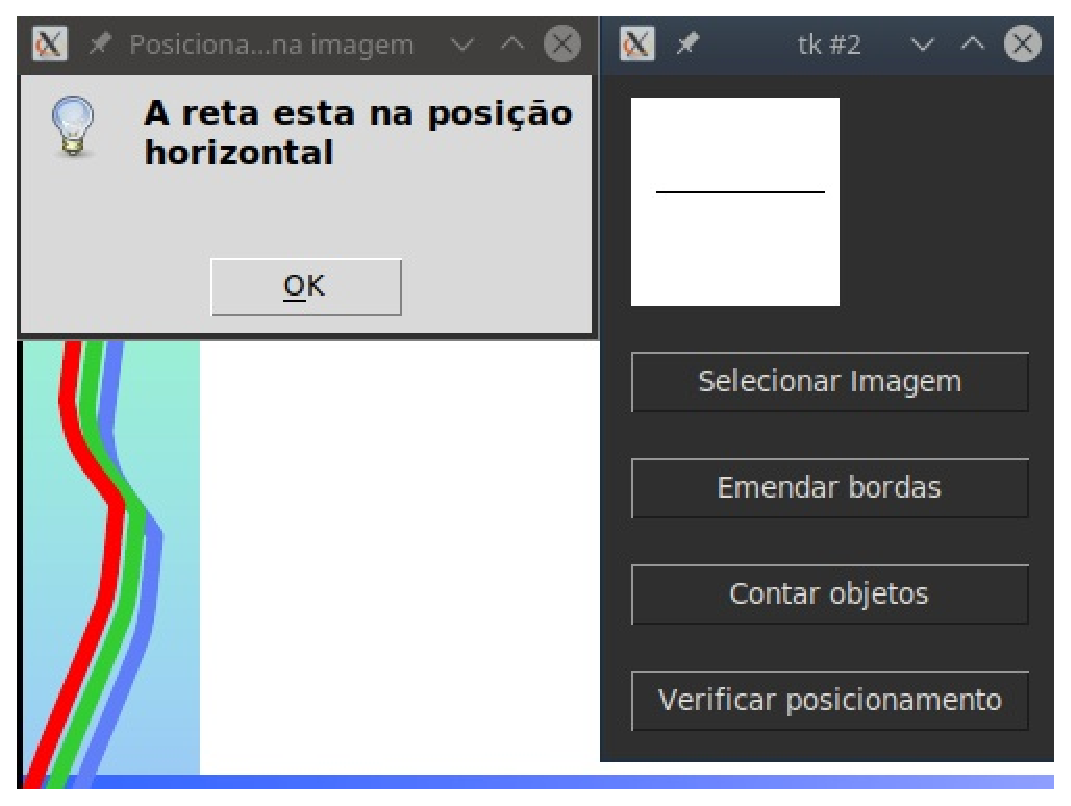
\includegraphics[scale=0.80]{cap_1.eps}
  \caption{Interface com resultado de execução da função de posicionamento}
\end{figure}

\pagebreak

\section{Quantidade de objetos}
\subsection{Código fonte}
\begin{python}
def quantidade_objetos(matriz_pixels):
    altura, largura = matriz_pixels.shape[0:2]
    matriz_flag = np.zeros((altura, largura), dtype='i')
    num_objetos = 0
    for linha in range(0, altura):
        for coluna in range(0, largura):
          if matriz_pixels[linha][coluna][0] != 255 and
           matriz_flag[linha][coluna] != 1:
              num_objetos += 1
              flag_regiao( linha, coluna, matriz_pixels, matriz_flag)
    return num_objetos

def flag_regiao(linha, coluna, matriz_pixels, matriz_flag):
    altura, largura = matriz_flag.shape[0:2]
    if linha == altura or coluna == largura or coluna < 0 or linha < 0:
        return 0
    elif matriz_pixels[linha][coluna][0] == 255 or matriz_flag[linha][coluna] == 1:
        return 0
    else:
        matriz_flag[linha][coluna] = 1
        flag_regiao( linha, coluna+1, matriz_pixels, matriz_flag)
        flag_regiao( linha+1, coluna+1, matriz_pixels, matriz_flag)
        flag_regiao( linha+1, coluna, matriz_pixels, matriz_flag)
        flag_regiao( linha, coluna-1, matriz_pixels, matriz_flag)
        flag_regiao( linha+1, coluna-1, matriz_pixels, matriz_flag)
        flag_regiao( linha-1, coluna, matriz_pixels, matriz_flag)
        flag_regiao( linha-1, coluna-1, matriz_pixels, matriz_flag)
        flag_regiao( linha-1, coluna+1, matriz_pixels, matriz_flag)
\end{python}
\subsection{Exemplo de processamento}
\paragraph{}
\begin{figure}[!h]
  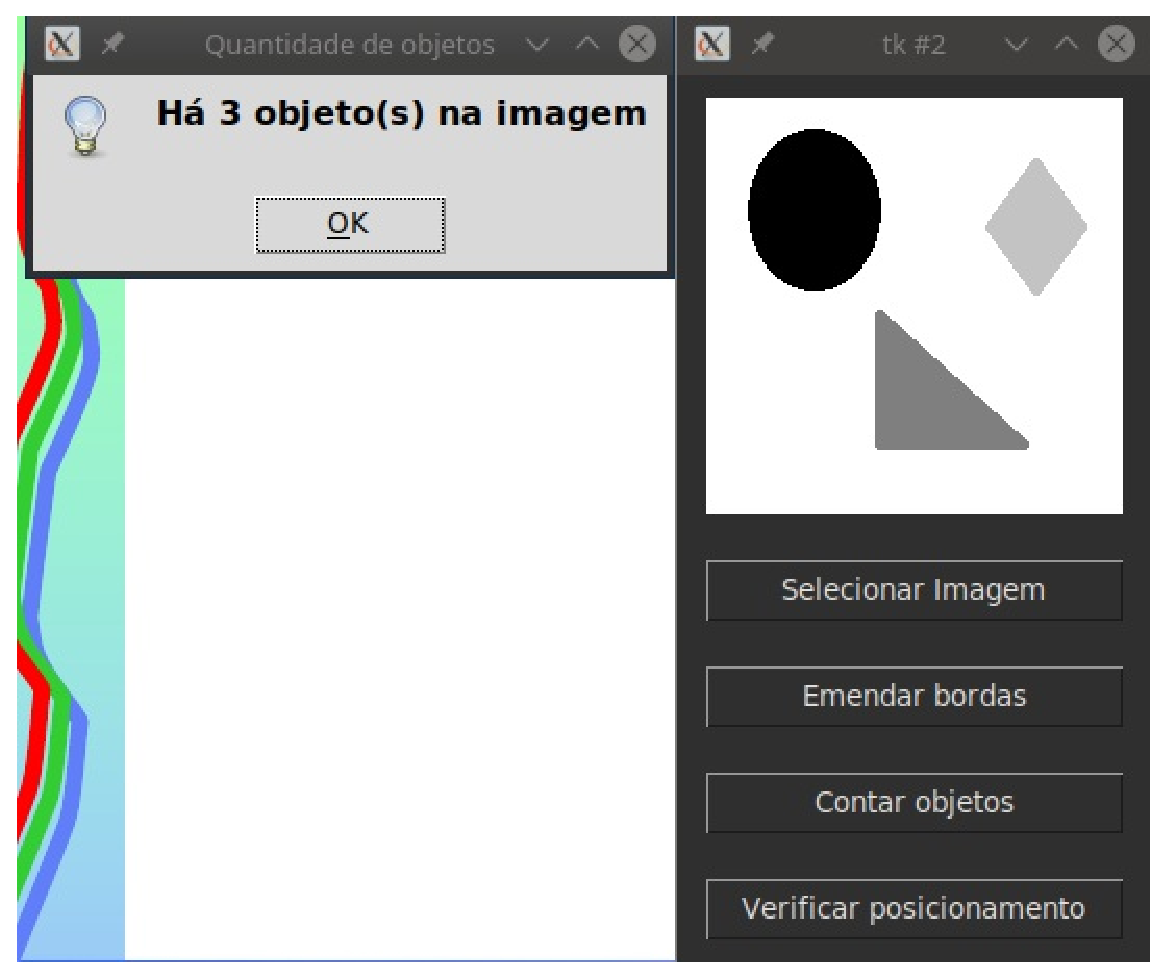
\includegraphics[scale=0.70]{cap_2.eps}
  \caption{Interface com resultado de execução da chamada a função de contagem}
\end{figure}

\section{Bordas}
\subsection{Código fonte}
\subsubsection{A)}
\begin{python}
def filtro_mediana(matriz_pixels):
   altura, largura = matriz_pixels.shape[0:2]
   nova_matriz_pixels = np.zeros((altura, largura))
   vizinhos_canais = np.zeros((1, 8))
   for linha in range(1, altura-1):
     for coluna in range(1, largura-1):
       vizinhos_canais[0][0] = copiar(matriz_pixels[linha-1][coluna-1][0])
       vizinhos_canais[0][1] = copiar(matriz_pixels[linha-1][coluna][0])
       vizinhos_canais[0][2] = copiar(matriz_pixels[linha-1][coluna+1][0])
       vizinhos_canais[0][3] = copiar(matriz_pixels[linha][coluna-1][0])
       vizinhos_canais[0][4] = copiar(matriz_pixels[linha][coluna+1][0])
       vizinhos_canais[0][5] = copiar(matriz_pixels[linha+1][coluna-1][0])
       vizinhos_canais[0][6] = copiar(matriz_pixels[linha+1][coluna][0])
       vizinhos_canais[0][7] = copiar(matriz_pixels[linha+1][coluna+1][0])
       vizinhos_canais = np.sort(vizinhos_canais)
       nova_matriz_pixels[linha][coluna] = copiar(vizinhos_canais[0][3])
   return nova_matriz_pixels.astype('uint8')
\end{python}
\subsubsection{B)}
\begin{python}
def borda_diferenciacao(matriz_pixels):
   altura, largura = matriz_pixels.shape[0:2]
   matriz_bordas = np.zeros((altura, largura), dtype='i')
   for linha in range(0, altura-1):
     for coluna in range(0, largura-1):
       realce = abs(matriz_pixels[linha][coluna]
        - matriz_pixels[linha+1][coluna]) + abs(matriz_pixels[linha][coluna]
        - matriz_pixels[linha][coluna+1])
       if realce > 150:
         matriz_bordas[linha][coluna] = 255
   return matriz_bordas.astype('uint8')
\end{python}
\subsubsection{C)}
\begin{python}
def ligacao(matriz_pixels):
  altura, largura = matriz_pixels.shape[0:2]
  matriz_ligada = np.copy(matriz_pixels)
  t = 25
  alfa_radianos = math.radians(80)
  angulo = alfa_radianos
  primeiro = False
  segundo = False
  for linha in range(0, altura-1):
    for coluna in range(0, largura-1):
      if sem_vizinho(linha, coluna, matriz_pixels):
        if primeiro == False:
          primeiro = True
          primeiro_X = linha
          primeiro_Y = coluna
          primeiro_GX = abs(matriz_pixels[linha][coluna]
           - matriz_pixels[linha+1][coluna])
          primeiro_GY = abs(matriz_pixels[linha][coluna]
           - matriz_pixels[linha][coluna+1])
        elif segundo == False:
          segundo = True
          segundo_X = linha
          segundo_Y = coluna
          segundo_GX = abs(matriz_pixels[linha][coluna]
           - matriz_pixels[linha+1][coluna])
          segundo_GY = abs(matriz_pixels[linha][coluna]
           - matriz_pixels[linha][coluna+1])
        if primeiro and segundo:
          magnitude = (primeiro_GX + primeiro_GY) - (segundo_GX + segundo_GY)
          if magnitude <= t:
            primeiro_angulo =  math.atan2(primeiro_GY, primeiro_GX) #radianos
            segundo_angulo =  math.atan2(segundo_GY, segundo_GX)
            angulo = abs(primeiro_angulo - segundo_angulo)
            if angulo < alfa_radianos:
              biblimagem.line(matriz_ligada,(primeiro_X, primeiro_Y),
               (segundo_X, segundo_Y),(255))
              primeiro = False
              segundo = False
              primeiro_GX = -1
              primeiro_GY = -1
              segundo_GX = -1
              segundo_GY = -1
            else:
              primeiro_GX = segundo_GX
              primeiro_GY = segundo_GY
              primeiro_X = segundo_X
              primeiro_Y = segundo_Y
              segundo = False
              segundo_GX = -1
              segundo_GY = -1
          else:
            primeiro_GX = segundo_GX
            primeiro_GY = segundo_GY
            primeiro_X = segundo_X
            primeiro_Y = segundo_Y
            segundo = False
            segundo_GX = -1
            segundo_GY = -1
  return matriz_ligada.astype('uint8')

def sem_vizinho(linha, coluna, matriz_pixels):
   altura, largura = matriz_pixels.shape[0:2]
   if linha == altura and coluna == largura:
       return 0
   else:
       contador = 0
       if matriz_pixels[linha-1][coluna-1] != 0:
           contador += 1
       if matriz_pixels[linha+1][coluna+1] != 0:
           contador += 1
       if matriz_pixels[linha-1][coluna+1] != 0:
           contador += 1
       if matriz_pixels[linha+1][coluna-1] != 0:
           contador += 1
       if matriz_pixels[linha][coluna-1] != 0:
           contador += 1
       if matriz_pixels[linha][coluna+1] != 0:
           contador += 1
       if matriz_pixels[linha-1][coluna] != 0:
           contador += 1
       if matriz_pixels[linha+1][coluna] != 0:
           contador += 1
       if contador < 2:
           return 1
       else:
           return 0
\end{python}

\subsection{Exemplo de processamento}
\begin{figure}[h!]
  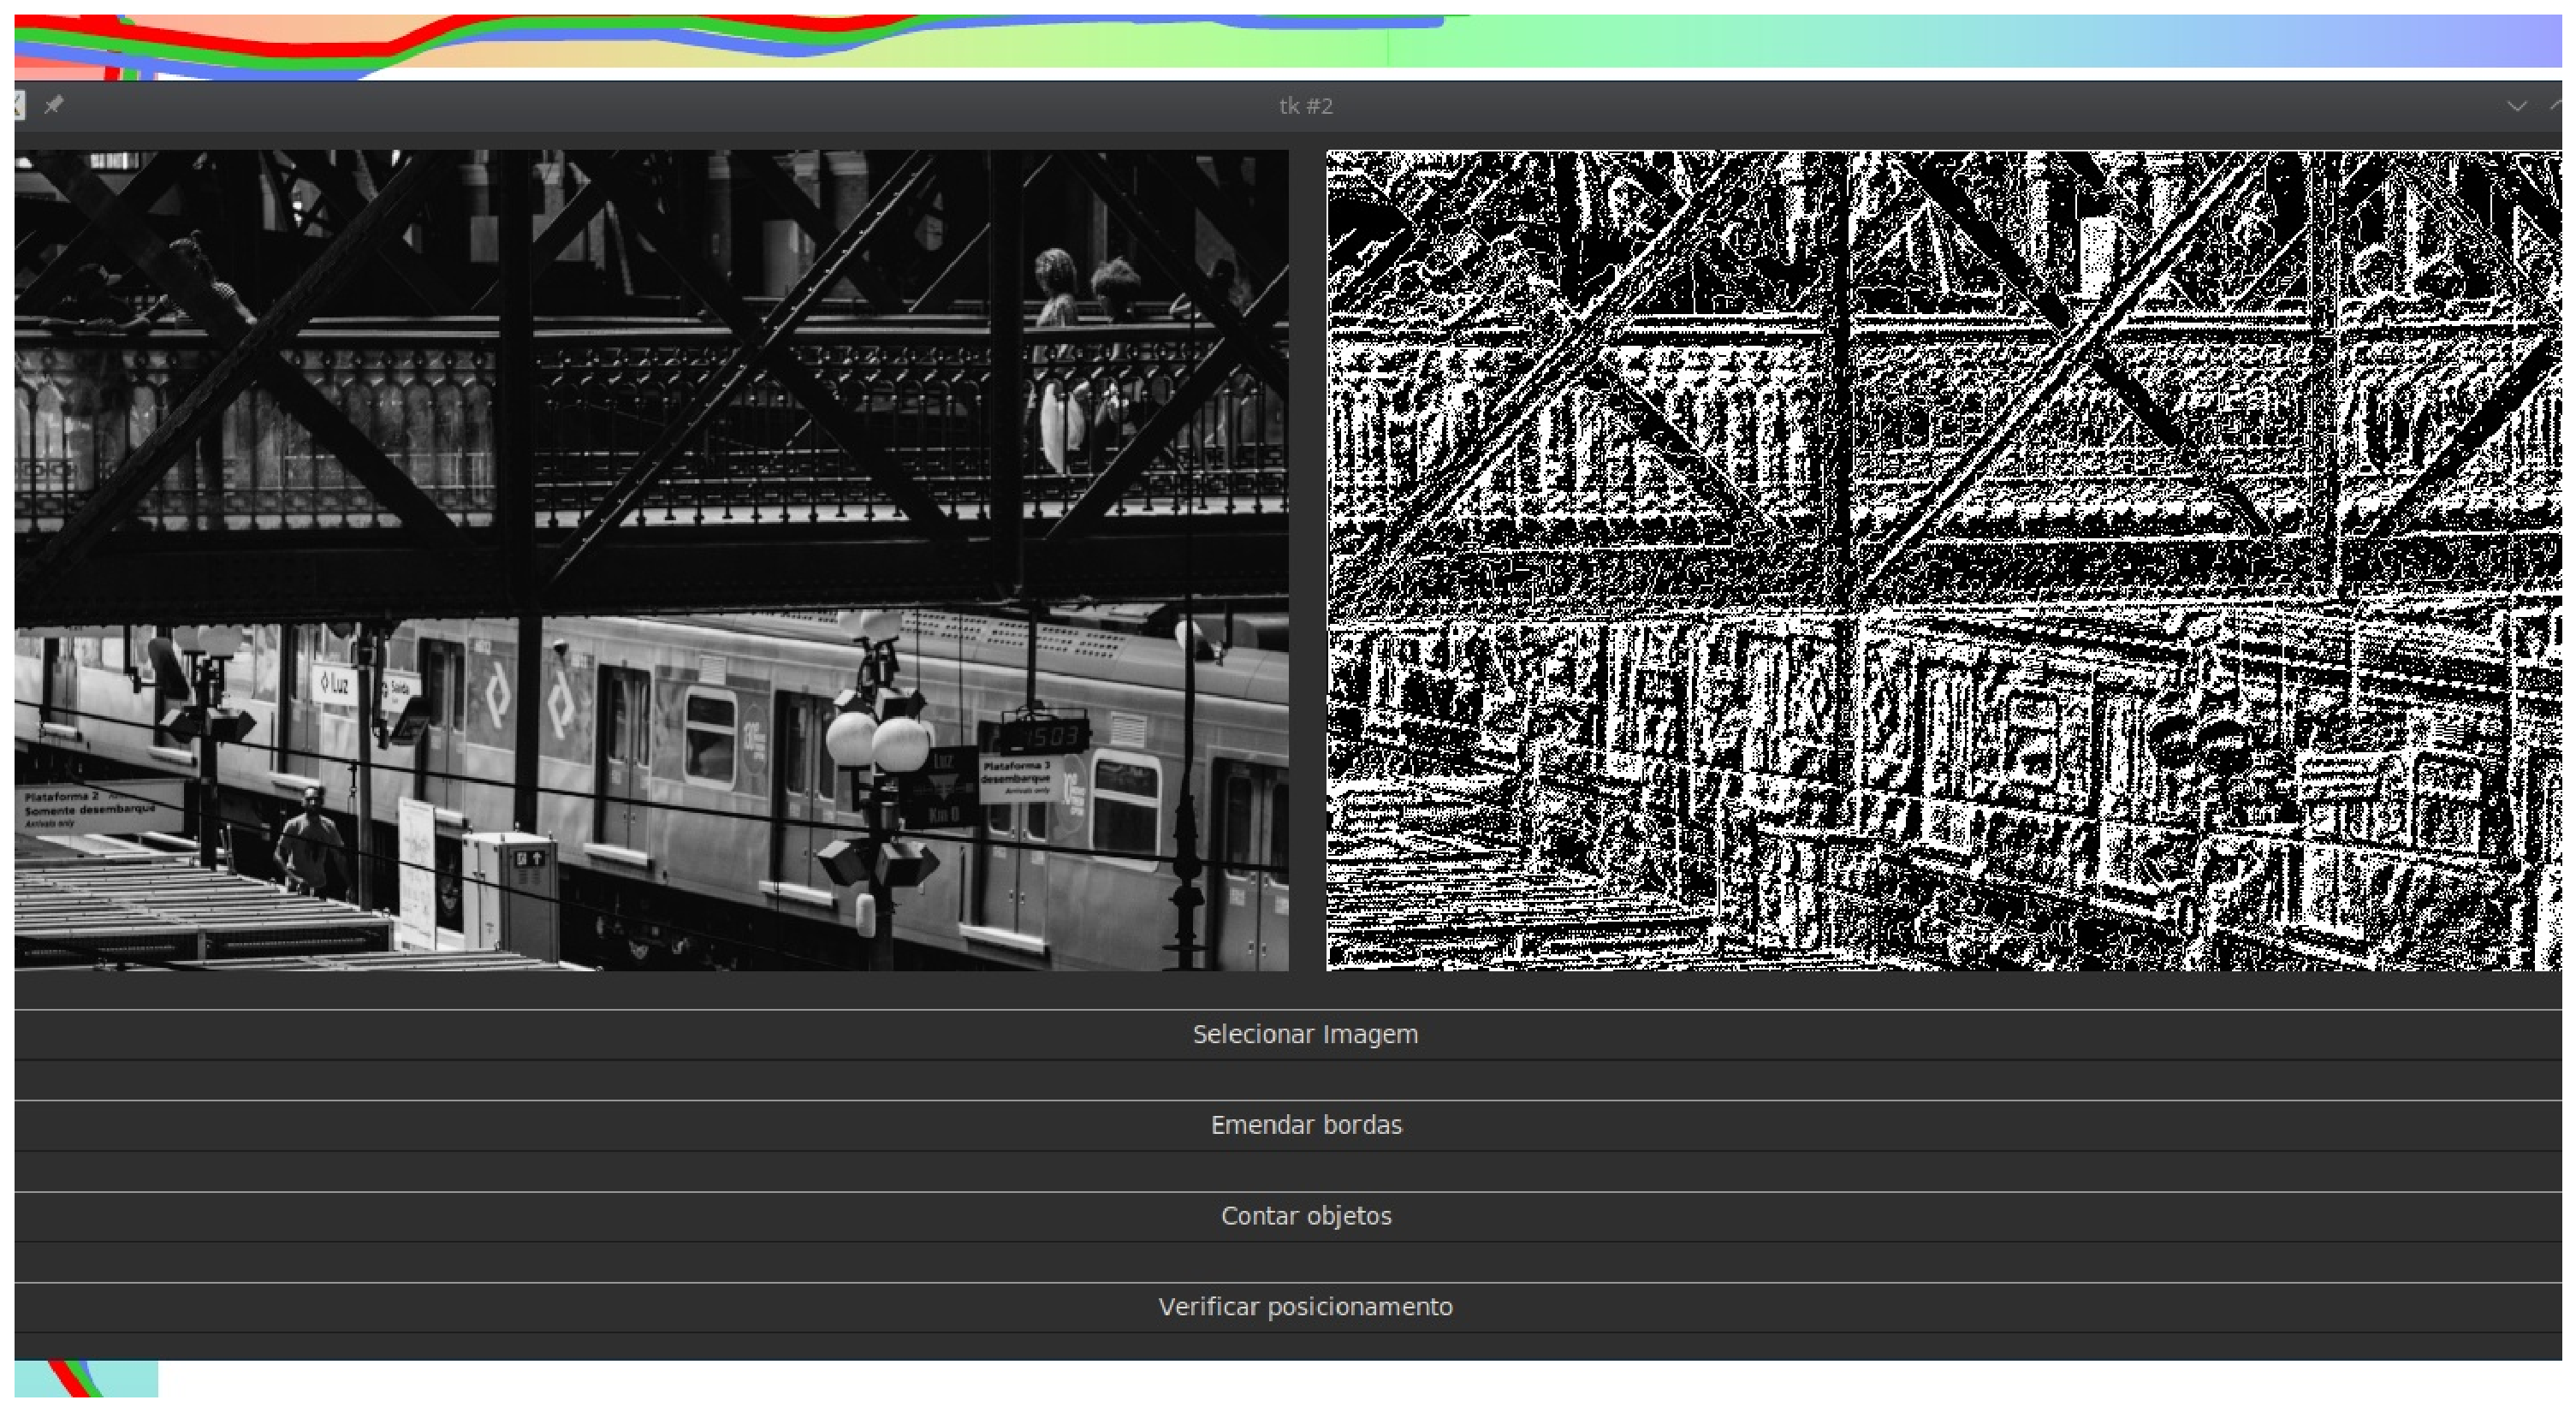
\includegraphics[scale=0.25]{cap_3.eps} \\
  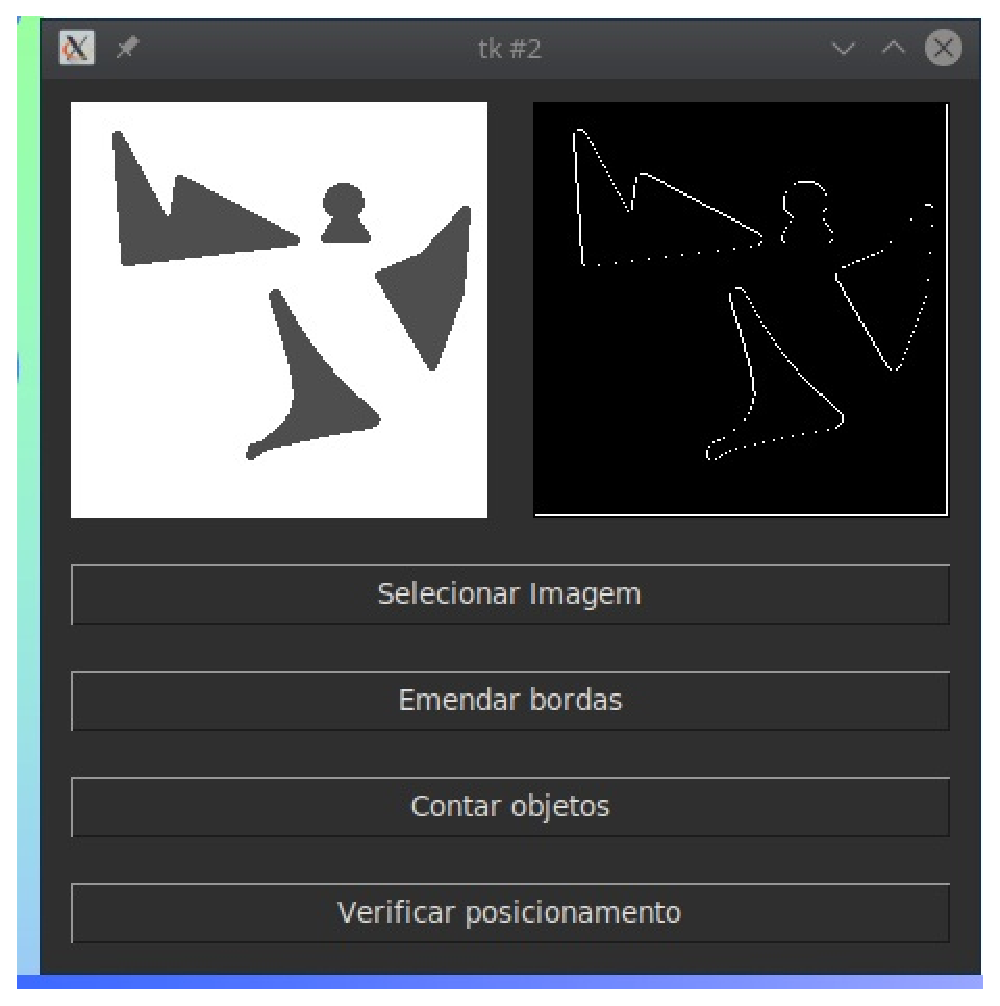
\includegraphics[scale=0.5]{cap_4.eps}
  \caption{Interface com resultado de execução da chamada das funções (A) e (B)}
\end{figure}

\end{document}